\section{Implementation}
In the previous section we introduced the Alpha algorithm and taken assumptions which were transformed into a timed automaton. The former description should be complete enough to implement Alpha algorithm with any suitable tool of choice. In this section we will focus on implementation with regards to the specific tool of our choice, UPPAAL. As the previous section finished on timed automaton, we will start by presenting timed automaton implemented in UPPAAL. We will draw connections between them as presented in Figure \ref{fig:automaton} and Figure \ref{fig:automaton_uppaal}. Then, we will explain global functions and state.

\begin{figure}[H]
\caption{UPPAAL implementation of the automaton}
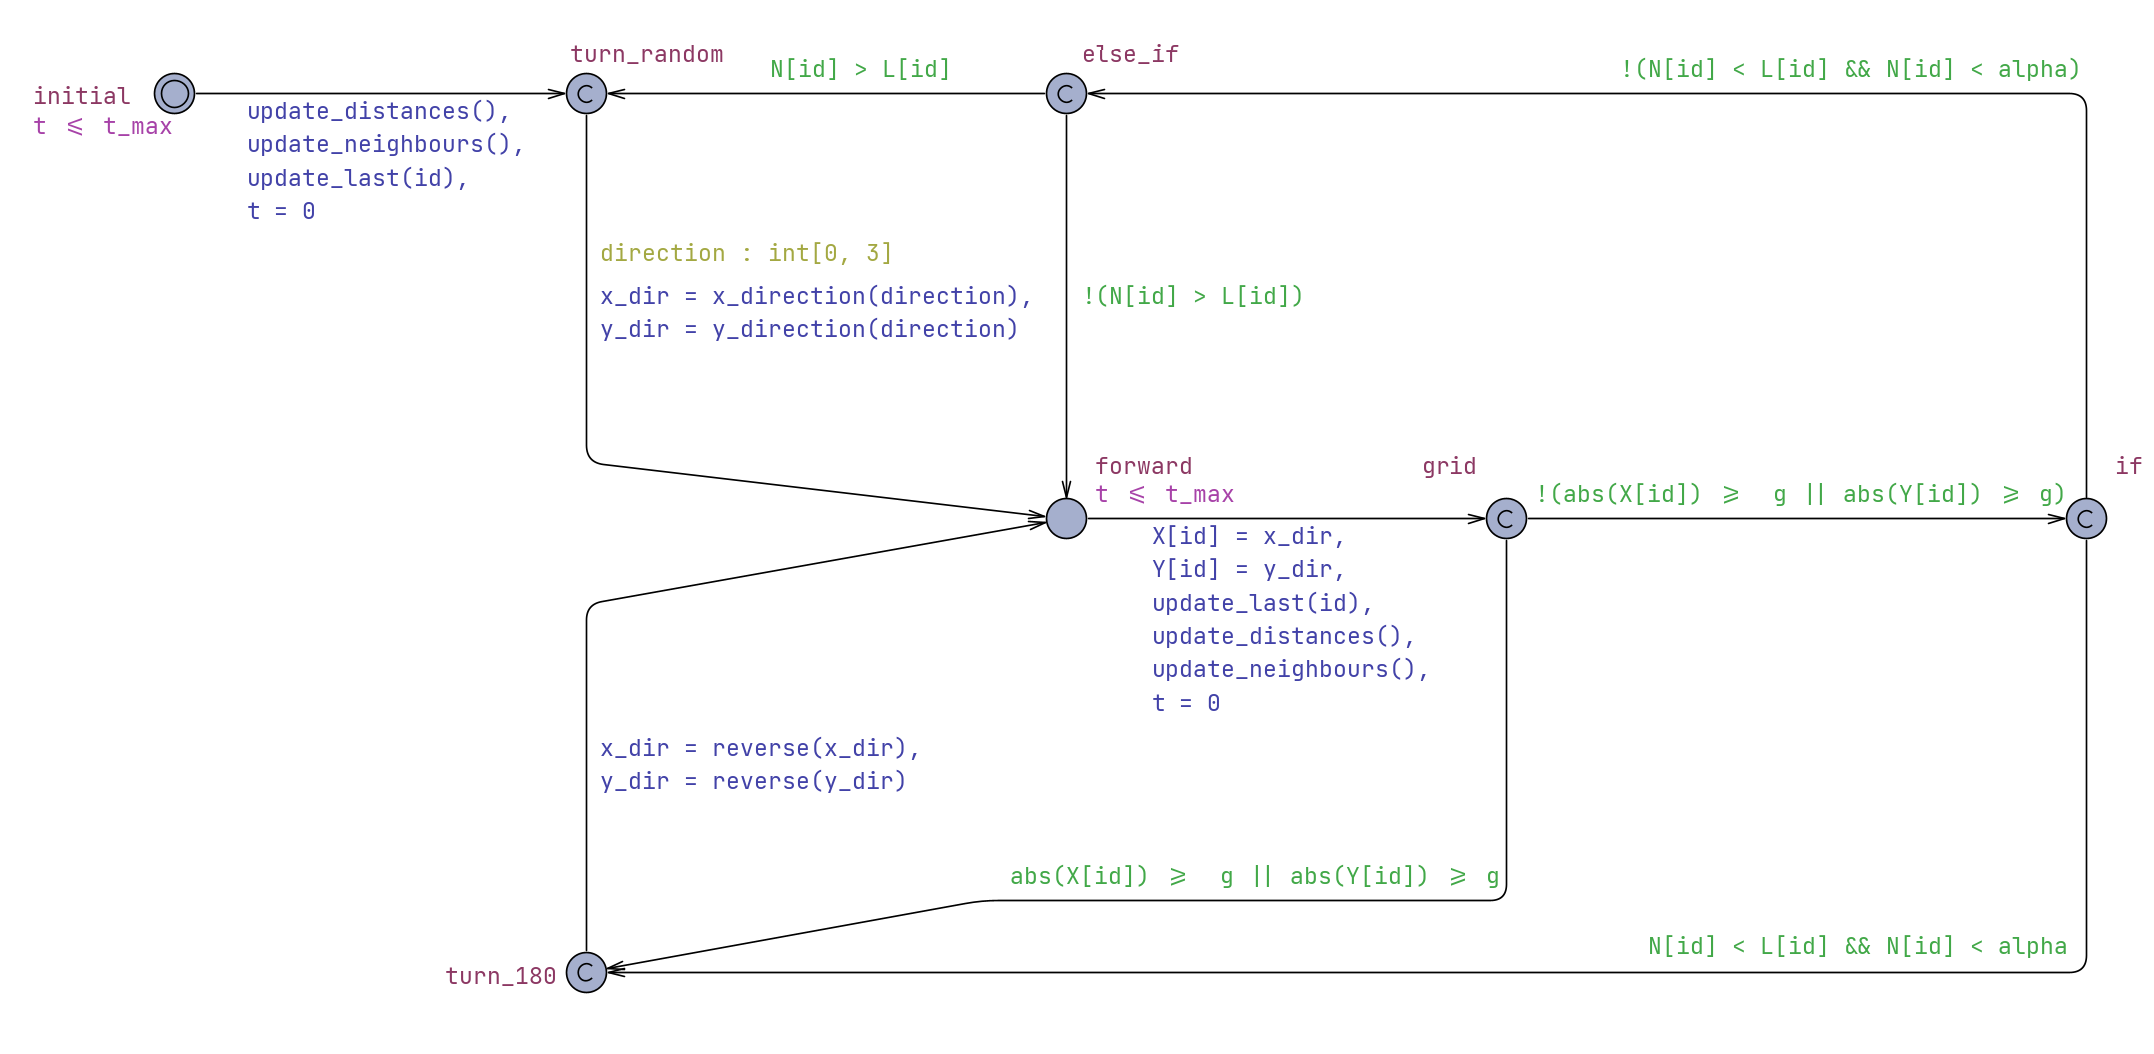
\includegraphics[scale=0.3]{images/automaton_uppaal.png}
\label{fig:automaton_uppaal}
\end{figure}

To start with comparison between general automaton and its specific implementation in UPPAAL, let's notice that both automata have the same set of states and transitions. Guarded transitions use the same conditions. Each robot accesses its own set of condition variables by providing \textbf{id} to the global arrays. Array \textbf{N} holds the number of neighbours for each robot. Array \textbf{L} holds the last number of neighbours for each robot. Those variables are held in the global arrays so that a single robot could update the number of neighbours for all of the other robots every time it moves. It may seem counter intuitive that a single robot updates the variables of other robots. However, the execution of the system composed from multiple robots is based on interleavings. At any given time a single robot transitions between states. This means that only the moving robot is guaranteed to have true information about number connections. Global updates of the number of neighbours is a way to mimic physical, continuous signal that would determine whether robots are connected or not. It eliminates the situation where robot would make a decision on already outdated information. The implementation assumes that each time a robot moves it will update its coordinates, update the last number of neighbours for itself and update the current number of neighbours for all robots. It achieves the last two actions by calling \textbf{update\_last(id)} and \textbf{update\_neighbours()}. Figure \ref{fig:neighbours} shows the process of updating the number of connections for all robots.
\begin{figure}[H]
\caption{Implementation of \textbf{update\_neighbours()} and \textbf{neighbours()}}
\lstset { language=C++ }
\begin{lstlisting}
int neighbours(int id){
    // returns the number of connections for a robot with a given id
    int x = X[id];  // x coordinate
    int y = Y[id];  // y coordinate
    int k = 0;      // neighbour counter k
    int i = 0;   
    for (i = 0; i < n; i++){
        double d = distance(x, y, X[i], Y[i]);
        bool c = connected(d);
        // is robot connected to another robot
        if(i != id && c){
            k++;
        }
    }
    return k;
}

void update_neighbours(){
    // updates the array that stores number of neighbours for each robot
    int i;
    for (i = 0; i < n; i++){
        N[i] = neighbours(i);
    }
}
\end{lstlisting}
\label{fig:neighbours}
\end{figure}

The number of connections will then determine the next transitions. Transition that is forced by the clock in the \textbf{forward} state will always result in the robot moving by a unit step in its current direction. Then based, on logical value of the conditions guarding transitions, it can also change its direction. The direction will change after robot reaches and transitions from states \textbf{turn\_random} or \textbf{turn\_180}. The random turn is realised as a random choice between four directions: up, right, down, up and translating it into x, y coordinates. The 180 degree turn is realised as choosing the opposite direction to the current one. Change of direction is achieved by functions \textbf{x\_direction(direction)}, \textbf{y\_direction(direction)}, \textbf{reverse(direction)}. Figure \ref{fig:direction} show the process of changing direction.
\begin{figure}[H]
\caption{Implementation of \textbf{x\_direction(direction)} and \textbf{reverse(direction)}}
\lstset { language=C++ }
\begin{lstlisting}
int x_direction(int direction){
    // maps direction to x axis
    if (direction == 1){
        // right
        return 1;
    }
    if (direction == 3){
        // left
        return -1;
    }
    // neither
    return 0;
}

int reverse(int direction){
    // reverses direction
    return direction * -1;
}
\end{lstlisting}
\label{fig:direction}
\end{figure}

The last element of the implementation is time. Each robot has its own clock that limits how long it can stay in the states with defined invariants: \textbf{initial}, \textbf{forward}. After transitioning from those states, a robot will reset its clock. Only in those states, the time passes. Other states are so called committed locations. In committed locations time doesn't pass which means that individual robot clocks do not progress. As a consequence the time progresses during the forward motion of the robot but decision to turn happens instantaneously.

We started from general timed automaton implementing the Alpha algorithm. We implemented it using UPPAAL and recreated states, transitions and conditions. We explained the reasoning behind using the global state for condition variables and the mechanism of updating them. We showed how the robot movement and changes of directions are realised and when it happens. Finally we described the timing aspect and its practical implications on the behaviour of the model.